\documentclass[twoside]{book}

% Packages required by doxygen
\usepackage{fixltx2e}
\usepackage{calc}
\usepackage{doxygen}
\usepackage[export]{adjustbox} % also loads graphicx
\usepackage{graphicx}
\usepackage[utf8]{inputenc}
\usepackage{makeidx}
\usepackage{multicol}
\usepackage{multirow}
\PassOptionsToPackage{warn}{textcomp}
\usepackage{textcomp}
\usepackage[nointegrals]{wasysym}
\usepackage[table]{xcolor}

% Font selection
\usepackage[T1]{fontenc}
\usepackage[scaled=.90]{helvet}
\usepackage{courier}
\usepackage{amssymb}
\usepackage{sectsty}
\renewcommand{\familydefault}{\sfdefault}
\allsectionsfont{%
  \fontseries{bc}\selectfont%
  \color{darkgray}%
}
\renewcommand{\DoxyLabelFont}{%
  \fontseries{bc}\selectfont%
  \color{darkgray}%
}
\newcommand{\+}{\discretionary{\mbox{\scriptsize$\hookleftarrow$}}{}{}}

% Page & text layout
\usepackage{geometry}
\geometry{%
  a4paper,%
  top=2.5cm,%
  bottom=2.5cm,%
  left=2.5cm,%
  right=2.5cm%
}
\tolerance=750
\hfuzz=15pt
\hbadness=750
\setlength{\emergencystretch}{15pt}
\setlength{\parindent}{0cm}
\setlength{\parskip}{3ex plus 2ex minus 2ex}
\makeatletter
\renewcommand{\paragraph}{%
  \@startsection{paragraph}{4}{0ex}{-1.0ex}{1.0ex}{%
    \normalfont\normalsize\bfseries\SS@parafont%
  }%
}
\renewcommand{\subparagraph}{%
  \@startsection{subparagraph}{5}{0ex}{-1.0ex}{1.0ex}{%
    \normalfont\normalsize\bfseries\SS@subparafont%
  }%
}
\makeatother

% Headers & footers
\usepackage{fancyhdr}
\pagestyle{fancyplain}
\fancyhead[LE]{\fancyplain{}{\bfseries\thepage}}
\fancyhead[CE]{\fancyplain{}{}}
\fancyhead[RE]{\fancyplain{}{\bfseries\leftmark}}
\fancyhead[LO]{\fancyplain{}{\bfseries\rightmark}}
\fancyhead[CO]{\fancyplain{}{}}
\fancyhead[RO]{\fancyplain{}{\bfseries\thepage}}
\fancyfoot[LE]{\fancyplain{}{}}
\fancyfoot[CE]{\fancyplain{}{}}
\fancyfoot[RE]{\fancyplain{}{\bfseries\scriptsize Generated by Doxygen }}
\fancyfoot[LO]{\fancyplain{}{\bfseries\scriptsize Generated by Doxygen }}
\fancyfoot[CO]{\fancyplain{}{}}
\fancyfoot[RO]{\fancyplain{}{}}
\renewcommand{\footrulewidth}{0.4pt}
\renewcommand{\chaptermark}[1]{%
  \markboth{#1}{}%
}
\renewcommand{\sectionmark}[1]{%
  \markright{\thesection\ #1}%
}

% Indices & bibliography
\usepackage{natbib}
\usepackage[titles]{tocloft}
\setcounter{tocdepth}{3}
\setcounter{secnumdepth}{5}
\makeindex

% Hyperlinks (required, but should be loaded last)
\usepackage{ifpdf}
\ifpdf
  \usepackage[pdftex,pagebackref=true]{hyperref}
\else
  \usepackage[ps2pdf,pagebackref=true]{hyperref}
\fi
\hypersetup{%
  colorlinks=true,%
  linkcolor=blue,%
  citecolor=blue,%
  unicode%
}

% Custom commands
\newcommand{\clearemptydoublepage}{%
  \newpage{\pagestyle{empty}\cleardoublepage}%
}

\usepackage{caption}
\captionsetup{labelsep=space,justification=centering,font={bf},singlelinecheck=off,skip=4pt,position=top}

%===== C O N T E N T S =====

\begin{document}

% Titlepage & ToC
\hypersetup{pageanchor=false,
             bookmarksnumbered=true,
             pdfencoding=unicode
            }
\pagenumbering{alph}
\begin{titlepage}
\vspace*{7cm}
\begin{center}%
{\Large Lab1 Project \\[1ex]\large 1.\+0 }\\
\vspace*{1cm}
{\large Generated by Doxygen 1.8.13}\\
\end{center}
\end{titlepage}
\clearemptydoublepage
\pagenumbering{roman}
\tableofcontents
\clearemptydoublepage
\pagenumbering{arabic}
\hypersetup{pageanchor=true}

%--- Begin generated contents ---
\chapter{Data Structure Index}
\section{Class List}
Here are the classes, structs, unions and interfaces with brief descriptions\+:\begin{DoxyCompactList}
\item\contentsline{section}{\hyperlink{classSemaphore}{Semaphore} \\*A \hyperlink{classSemaphore}{Semaphore} Implementation }{\pageref{classSemaphore}}{}
\end{DoxyCompactList}

\chapter{File Index}
\section{File List}
Here is a list of all files with brief descriptions\+:\begin{DoxyCompactList}
\item\contentsline{section}{/home/ger/\+Desktop/\+C\+D\+D\+Labs/\+Lab1/\hyperlink{_semaphore_8cpp}{Semaphore.\+cpp} }{\pageref{_semaphore_8cpp}}{}
\item\contentsline{section}{/home/ger/\+Desktop/\+C\+D\+D\+Labs/\+Lab1/\hyperlink{_semaphore_8h}{Semaphore.\+h} }{\pageref{_semaphore_8h}}{}
\item\contentsline{section}{/home/ger/\+Desktop/\+C\+D\+D\+Labs/\+Lab1/\hyperlink{signal_8cpp}{signal.\+cpp} }{\pageref{signal_8cpp}}{}
\end{DoxyCompactList}

\chapter{Data Structure Documentation}
\hypertarget{classSemaphore}{}\section{Semaphore Class Reference}
\label{classSemaphore}\index{Semaphore@{Semaphore}}


A \hyperlink{classSemaphore}{Semaphore} Implementation.  




{\ttfamily \#include $<$Semaphore.\+h$>$}

\subsection*{Public Member Functions}
\begin{DoxyCompactItemize}
\item 
\mbox{\Hypertarget{classSemaphore_a0d9290d316636875ca85d1d78950a817}\label{classSemaphore_a0d9290d316636875ca85d1d78950a817}} 
{\bfseries Semaphore} (unsigned int ui\+Count=0)
\item 
\mbox{\Hypertarget{classSemaphore_a72aabebf026e3a8b1f3e4d0fa8ee1eda}\label{classSemaphore_a72aabebf026e3a8b1f3e4d0fa8ee1eda}} 
void {\bfseries Wait} ()
\item 
\mbox{\Hypertarget{classSemaphore_a7f700173ae86ae623684109066e07656}\label{classSemaphore_a7f700173ae86ae623684109066e07656}} 
{\footnotesize template$<$typename R , typename P $>$ }\\bool {\bfseries Wait} (const std\+::chrono\+::duration$<$ R, P $>$ \&cr\+Rel\+Time)
\item 
\mbox{\Hypertarget{classSemaphore_a86f92f738b4486439b296d8e235895f2}\label{classSemaphore_a86f92f738b4486439b296d8e235895f2}} 
void {\bfseries Signal} ()
\end{DoxyCompactItemize}


\subsection{Detailed Description}
A \hyperlink{classSemaphore}{Semaphore} Implementation. 

\begin{DoxyAuthor}{Author}
Ger Dobbs 
\end{DoxyAuthor}
\begin{DoxyDate}{Date}
02/10/2017 
\end{DoxyDate}
\begin{DoxyVersion}{Version}
1.\+0
\end{DoxyVersion}
Uses C++11 features such as mutex and condition variables to implement \hyperlink{classSemaphore}{Semaphore} 

The documentation for this class was generated from the following files\+:\begin{DoxyCompactItemize}
\item 
Semaphore.\+h\item 
Semaphore.\+cpp\end{DoxyCompactItemize}

\chapter{File Documentation}
\hypertarget{Semaphore_8cpp}{}\section{Semaphore.\+cpp File Reference}
\label{Semaphore_8cpp}\index{Semaphore.\+cpp@{Semaphore.\+cpp}}
{\ttfamily \#include \char`\"{}Semaphore.\+h\char`\"{}}\newline
Include dependency graph for Semaphore.\+cpp\+:
\nopagebreak
\begin{figure}[H]
\begin{center}
\leavevmode
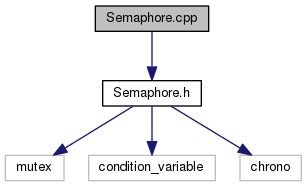
\includegraphics[width=302pt]{Semaphore_8cpp__incl}
\end{center}
\end{figure}

\hypertarget{Semaphore_8h}{}\section{Semaphore.\+h File Reference}
\label{Semaphore_8h}\index{Semaphore.\+h@{Semaphore.\+h}}
{\ttfamily \#include $<$mutex$>$}\newline
{\ttfamily \#include $<$condition\+\_\+variable$>$}\newline
{\ttfamily \#include $<$chrono$>$}\newline
Include dependency graph for Semaphore.\+h\+:
\nopagebreak
\begin{figure}[H]
\begin{center}
\leavevmode
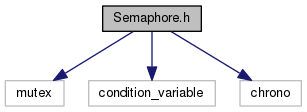
\includegraphics[width=302pt]{Semaphore_8h__incl}
\end{center}
\end{figure}
This graph shows which files directly or indirectly include this file\+:
\nopagebreak
\begin{figure}[H]
\begin{center}
\leavevmode
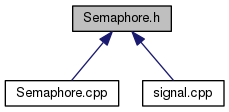
\includegraphics[width=244pt]{Semaphore_8h__dep__incl}
\end{center}
\end{figure}
\subsection*{Classes}
\begin{DoxyCompactItemize}
\item 
class \hyperlink{classSemaphore}{Semaphore}
\begin{DoxyCompactList}\small\item\em A \hyperlink{classSemaphore}{Semaphore} Implementation. \end{DoxyCompactList}\end{DoxyCompactItemize}

\hypertarget{signal_8cpp}{}\section{/home/ger/\+Desktop/\+C\+D\+D\+Labs/\+Lab1/signal.cpp File Reference}
\label{signal_8cpp}\index{/home/ger/\+Desktop/\+C\+D\+D\+Labs/\+Lab1/signal.\+cpp@{/home/ger/\+Desktop/\+C\+D\+D\+Labs/\+Lab1/signal.\+cpp}}
{\ttfamily \#include \char`\"{}Semaphore.\+h\char`\"{}}\newline
{\ttfamily \#include $<$iostream$>$}\newline
{\ttfamily \#include $<$thread$>$}\newline
\subsection*{Functions}
\begin{DoxyCompactItemize}
\item 
void \hyperlink{signal_8cpp_a2696073bbedb6b55e6a52d2180c2a9b3}{task\+One} (std\+::shared\+\_\+ptr$<$ \hyperlink{class_semaphore}{Semaphore} $>$ the\+Semaphore)
\item 
void \hyperlink{signal_8cpp_ae4ea9570be601d182fa473c7ca431852}{task\+Two} (std\+::shared\+\_\+ptr$<$ \hyperlink{class_semaphore}{Semaphore} $>$ the\+Semaphore)
\item 
int \hyperlink{signal_8cpp_a840291bc02cba5474a4cb46a9b9566fe}{main} (void)
\end{DoxyCompactItemize}


\subsection{Function Documentation}
\mbox{\Hypertarget{signal_8cpp_a840291bc02cba5474a4cb46a9b9566fe}\label{signal_8cpp_a840291bc02cba5474a4cb46a9b9566fe}} 
\index{signal.\+cpp@{signal.\+cpp}!main@{main}}
\index{main@{main}!signal.\+cpp@{signal.\+cpp}}
\subsubsection{\texorpdfstring{main()}{main()}}
{\footnotesize\ttfamily int main (\begin{DoxyParamCaption}\item[{void}]{ }\end{DoxyParamCaption})}

$<$ Launch the threads 

Definition at line 26 of file signal.\+cpp.

\mbox{\Hypertarget{signal_8cpp_a2696073bbedb6b55e6a52d2180c2a9b3}\label{signal_8cpp_a2696073bbedb6b55e6a52d2180c2a9b3}} 
\index{signal.\+cpp@{signal.\+cpp}!task\+One@{task\+One}}
\index{task\+One@{task\+One}!signal.\+cpp@{signal.\+cpp}}
\subsubsection{\texorpdfstring{task\+One()}{taskOne()}}
{\footnotesize\ttfamily void task\+One (\begin{DoxyParamCaption}\item[{std\+::shared\+\_\+ptr$<$ \hyperlink{class_semaphore}{Semaphore} $>$}]{the\+Semaphore }\end{DoxyParamCaption})}

\begin{DoxyAuthor}{Author}
Ger Dobbs 
\end{DoxyAuthor}
\begin{DoxyDate}{Date}
02/10/2017 
\end{DoxyDate}
\begin{DoxyVersion}{Version}
1.\+0 
\end{DoxyVersion}


Definition at line 11 of file signal.\+cpp.

\mbox{\Hypertarget{signal_8cpp_ae4ea9570be601d182fa473c7ca431852}\label{signal_8cpp_ae4ea9570be601d182fa473c7ca431852}} 
\index{signal.\+cpp@{signal.\+cpp}!task\+Two@{task\+Two}}
\index{task\+Two@{task\+Two}!signal.\+cpp@{signal.\+cpp}}
\subsubsection{\texorpdfstring{task\+Two()}{taskTwo()}}
{\footnotesize\ttfamily void task\+Two (\begin{DoxyParamCaption}\item[{std\+::shared\+\_\+ptr$<$ \hyperlink{class_semaphore}{Semaphore} $>$}]{the\+Semaphore }\end{DoxyParamCaption})}



Definition at line 18 of file signal.\+cpp.


%--- End generated contents ---

% Index
\backmatter
\newpage
\phantomsection
\clearemptydoublepage
\addcontentsline{toc}{chapter}{Index}
\printindex

\end{document}
